\ifsvnmulti
 \svnkwsave{$RepoFile: lyapunov/Henon.tex $}
 \svnidlong {$HeadURL: svn://zero.physics.gatech.edu/siminos/lyapunov/Henon.tex $}
 {$LastChangedDate: 2017-01-18 23:47:27 -0500 (Wed, 18 Jan 2017) $}
 {$LastChangedRevision: 5504 $} {$LastChangedBy: predrag $}
 \svnid{$Id: Henon.tex 5504 2017-01-19 04:47:27Z predrag $}
\fi

\chapter{H\'enon  attractor}
\label{c-Henon}

This chapter of the blog deals specifically with the
H\'enon attractor nonhyperbolicities.

%%-----   Qualitative dynamics, for cylists
\section{ChaosBook chapter: Stretch, fold, prune}
\label{c-smale}



\noindent
This section on the loan from ChaosBook.org,
dasbuch/book/chapter/smale.tex, to be edited here and eventually
returned. I have to write up pruning fronts anyway, if we can do it by
talking to each other it will be much more fun...

\Remarks

\remark{Pruning fronts / partition lines.}{\label{s_Henon_pruning}
                                                            \toCB
    \index{Henon@H\'enon map!pruning front}
% Predrag 2011-10-08: incorporated Dullin \etal\rf{HamSteDuMei04} remarks
A dynamical system is said to be \emph{hyperbolic} if its \statesp\ has
no homoclinic tangencies, \ie, the stable and unstable manifolds are
everywhere transversal to each other. The kneading theory\rf{MilThu88}
solves the problem of fully specifying the symbolic dynamics for
non-hyperbolic multimodal maps on a unit interval. The H\'enon mapping is
the springboard for generalization of the 1-\dmn\ theory to
higher-dimensional, nonhyperbolic systems.
        \PC{some useful bibTeX items can be found here:
    thesis.library.caltech.edu/2253/1/haha.bib,
    www.nahee.com/spanky/pub/fractals/docs/fractal.bib}

A \statesp\ partition that is too coarse assigns the same itinerary to
distinct dynamical trajectories. To avoid that, one works with partitions
finer than can be realized by the particular dynamical system. The
dynamics in the refined partition assigns a unique infinite itinerary $
\biinf{\Ssym{-2}\Ssym{-1}\Ssym{0}}{\Ssym{1}\Ssym{2} \Ssym{3}}$ to each
distinct orbit, but there might exist full shift symbol sequences
    \ifdasbuch
\refeq{FullSh}
    \else
    \fi
which are not realized as orbits; such sequences are called {\em
\inadmissible}. In \refref{AACI} the process of ferreting out the
{\em \inadmissible} sequences has given name {\em pruning}, descriptive of
pruning of branches corresponding to forbidden sequences for symbolic
dynamics, organized hierarchically into a tree structure\ifdasbuch,
as explained in \refchap{c-Markov}\else.
    \fi
\index{inadmissible symbol sequence}\index{symbol!sequence!inadmissible}
\index{pruning!symbolic dynamics}\index{symbolic dynamics!pruned}
    \PC{use this: `Pruning was introduced by Cvitanovi\'c to describe the
    topological dynamics of the H\'enon and Lozi families as partially
    formed horseshoes'}

In 1985 Grassberger and Kantz\rf{GK85} formulated the `partition conjecture'
    \ifdasbuch
    \PublicPrivate{}{
of \refsect{s-prunfront}
        }% end \PublicPrivate
    \else
    \fi
to describe the grammar of admissible binary itineraries for the H\'enon
map. Independently and concurrently, the equivalent concept of a `pruning
front' in the symbol plane and the `pruning-front conjecture' on its
monotonicity was formulated by Cvitanovi\'c \etal\rf{pre88top} in spring
1985. The idea behind these approaches is that the stable / unstable
manifolds foliation locks admissible itineraries in a rigid cage, and
that is suffices to specify the orbits of `primary' folds of the unstable
manifold in order to fully specify the symbolic dynamics of H\'enon and
Lozi type maps. For the logistic map admissible sequences are specified
by the itinerary of the critical point orbit, and the H\'enon map the are
determined by partitioning the symbol plane using the stable and unstable
foliation and their `primary homoclinic tangencies'.

The pruning front theory was applied by K.T.~Hansen to a number of
dynamical systems\rf{Hansen92b,Hansen92-1,Hansen92-2}. The `multimodal
map approximation' is described in the K.T.~Hansen thesis\rf{hansen}.
Hansen's Ph.D. thesis\rf{hansen} remains the most accessible exposition
of the pruning theory and its applications for a physicist. Symbol
sequences defined this way can morph into other sequences under
continuous changes of parameters\rf{hansen92}, and primary folds may
exhibit discontinuities\rf{GiPo92}.
    \PC{drop this: `This method
        has been applied to the cubic H\'enon map\rf{Fang94}?'}
Detailed studies of pruning fronts are carried out in
\refrefs{AlIsPo91,GiPo92,grass89}; \refref{AGIP90} is the most detailed
study carried out so far the H\'enon attractor, and Weibert
\etal\rf{WeiMaWu02} for a billiard.
    \PC{Is  \refref{AGIP90} the right one? Or should it be???}
The rigorous theory of pruning fronts has been developed by Y.
Ishii\rf{Ish97,Ishii97a} for the Lozi map, and A. de~Carvalho and
T.~Hall\rf{Carvalho99,CaHa01a,CaHa02} in a general and deep setting,
where it turns out be related to {Thurston}'s classification of surface
homeomorphisms\rf{CaHa01a}.

Several other methods have also been deployed to obtain H\'enon symbolic
dynamics. Hansen and Cvitanovi\'c\rf{hansen1d} approximate the
two-dimensional map by nested one-dimensional unimodal maps, but
the orbit code can change if it crosses the critical point of one of the
approximating maps. Biham and Wenzel\rf{afind} defined the codes as the
signature of a fictitious time descent gradient method for finding
periodic orbits\ifdasbuch
(see \refchap{c-relax})
    \else
    \fi,
and Sterling and Meiss\rf{StMeiss98} have shown that the method works
sufficiently close to an anti-integrable limit. Unfortunately, it does
not always converge to fixed points, and sometimes gives two codes for
the same orbit\rf{grass89}.

Beyond the orbit pruning and its infinity of \admissible\ unstable
orbits, an attractor of H\'enon type may also own an infinity of
attractive orbits coexisting with the strange
attractor\rf{nhouse74,nhouse79}. We offer heuristic arguments  and
numerical evidence that the coexistence of attractive orbits does not
destroy the strange attractor/repeller, which is also in this case
described by the 2\dmn\ danish pastry plot.

Pruning front technique have also been applied to the area-preserving
standard map by Dullin \etal(where is rf{HamSteDuMei04}?), among others. For large
$k$ parameter values where elliptic islands are small, Christiansen and
Politi\rf{chr95gen} have shown that a primary set of homoclinic
tangencies can be identified by their proximity to the dominant fold
lines in the map. Most impressively, the gaps between these points can be
connected with the reversibility symmetry lines to form a partition
line\rf{ChPo97} that partitions the elliptic islands\rf{ChPo96,ChPo97} as
well.
    \PC{refine references, emphasize Carvalho Nonlinearity review}
    \PC{
    Benedicks and Carleson\rf{BC89} have proven that
    in the vicinity of $(a,b)=(2,0)$ strange attractors exist for a
    Lebesgue measure in the parameter space.~PC: {recheck the phrasing!}
       }
    \PC{replace {CGP} $to$ pre88top,
    hansen\_thesis $\to$ hansen,
    Biham89 $\to$ afind,
    GKM $\to$ grass89,
     in all refs*tex}
} % end \remark{Pruning fronts.}{


\RemarksEnd

\begin{description}

\item[2010-10-07 Predrag]
                                                            \toCB
Mention anti-integrability and cite Aubry and Abramovici\rf{AuAb90}
and perhaps other Aubry papers\rf{AuDae83} when
discussing the chaotic trajectories in the standard map.

\item[2011-07-19 CS]
About Example 12.3 H\'enon repeller complete horseshoe:
First, in figure 12.4, why after one step's evolution, point B occupies
point D's original spot and also point C and point D are in the stable
manifold? I do not think this is just a coincidence but still haven't
figure out the reason.

\item[2011-07-22 CS] I read the Smale Horseshoe part in Kai's thesis. Now
I understand why the binary sequence has to be assigned this way. Only in
this way can the symbol represent the actual map. It's hard to describe
it but this picture found from wiki helped me a lot.

%%%%%%%%%%%%%%%%%%%%%%%%%%%%%%%%%%%%%%%%%%%%%%%%%%%%%%%%%%%%%%%%%%
\SFIG{SmaleHorseshoe} %{HMV}
{}{
This is a Smale horseshoe that I snitched from an unnamed wiki
without attribution. Cute, no?
    }{Fig:SmaleHorseshoe}
%%%%%%%%%%%%%%%%%%%%%%%%%%%%%%%%%%%%%%%%%%%%%%%%%%%%%%%%%%%%%%%%%

In Kai's thesis, he mentioned ``since the horseshoe is a diffeomorphism
we need to know both the future and the past.'' With the help of this
picture I kind of understand this.

Also I found something interesting that animates the procedure of H\'enon
map horseshoe:
\HREF{http://www.ibiblio.org/e-notes/Chaos/henon.htm}
{www.ibiblio.org/e-notes/Chaos/henon.htm}

\item[2011-07-23 PC]                                        \inCB
I had noticed Demidov's website before - you are right, these simulations
are very instructive, I have now added a remark about them to ChaosBook.
He uses a different definition for parameters $a$ and $b$ from H\'enon,
but unfortunately uses the same letters. His definition is natural if one
is interested in Julia sets, but unfortunately not the one H\'enon used,
and I always try to follow the foundational papers, rather than confusing
everybody with sly parameter redefinitions.


\item[2011-07-20 PC]                                        \toCB
Concerning the H\'enon attractor \underline{not} being symmetric across
the diagonal in general: check my
\HREF{http://chaosbook.org/version13/Maribor11.shtml}{Maribor lectures}.
In \HREF{http://chaosbook.org/overheads/dimension/dimension.pdf}{piece
\#5}: ``Dynamics in infinitely many dimensions'' slide 10 shows the
stable / unstable manifolds for the canonical H\'enon attractor - clearly
very asymmetric.

%%%%%%%%%%%%%%%%%%%%%%%%%%%%%%%%%%%%%%%%%%%%%%%%%%%%%%%%%%%%%%%%%%
\SFIG{Demidov_a-6_b-1}
{}{
PC: The Smale backward-forward horseshoe generated by the
Demidov\rf{DemChaos} java applets for the H\'enon parameter values
$(a,b) = (6,-1)$.
    }{Fig:Demidov}
%%%%%%%%%%%%%%%%%%%%%%%%%%%%%%%%%%%%%%%%%%%%%%%%%%%%%%%%%%%%%%%%%

\item[2011-07-24 PC]                                        \toCB
H\'enon's parametrization\rf{henon}:
\index{Henon@H\'enon map}
\index{map!H\'enon}
\bea
    x_{n+1}&=&1-ax^2_n+b y_n
        \continue
    y_{n+1}&=& x_n
\,.
\label{eq2.1a}
\eea
Demidov's parametrization\rf{DemChaos} of the H\'enon map is:
\bea
    x_{n+1}' &=& a'+ {x'}{}^2_n + b' y_n'
        \continue
    y_{n+1}' &=& x_n'
\,.
\label{DemidHen}
\eea
Dividing through by $a'$ we get
\(
\frac{x_{n+1}'}{a'} = 1 + a'\left(\frac{x_n'}{a'}\right)^2 + b'\frac{y_n'}{a'}
\,,
\)
so the two parametrizations are related by:
    \CS{my guess was
\[ %beq
x={x'}/{a'}
\,,\qquad
a=-{1}/{a'}
\,,\qquad b= {b'}/{a'}
\] %ee{DemidHenChao}
    }
\beq
x={x'}/{a'}
\,,\quad
y={y'}/{a'}
\,;\qquad
a=-{a'}
\,,\quad b= {b'}
\,.
\ee{DemidHenPar}
You need the transformation between two definitions, if you are
going to use Demidov's simulations to test your ideas, and it helps greatly
if the transformation formula is the correct one. If
I am right, if you chose
\(
a'=-6
\,,\quad
b'= -1
\)
Demidov's java applets reproduce the figures in ChaosBook?

\item[2012-07-23 PC]                                        \toCB
Refer to Mitchell\rf{Mitchell12}
{\em Partitioning two-dimensional mixed phase spaces}.

\item[2012-07-24 PC]                                        \toCB
Read Emilia Petrisor {\em Twist number and order properties of periodic orbits}
\arXiv{1105.4404}.

\item[2013-02-22 PC]                                        \toCB
J. Starrett and C. Nicholas\rf{StaNich12},
``A suspension of the {H\'enon} map by periodic orbits,''
does not cite our {H\'enon} articles. They have a list of
periodic points for \po s up to $\cl{}=7$. Crosscheck them.

\item[2013-06-19 PC]                                        \toCB
Check Mendoza\rf{Mendoza13} {\em Proof of the {Pruning Front Conjecture}
             for certain {H\'enon} parameters} for an up-to-date
status of the {Pruning Front Conjecture}.
He also cites Davis \etal\rf{DaMacKaSa1991}




\end{description}



\section{H\'enon blog}

\begin{description}

\item[2010-02-26 Predrag]
%
%%%%%%%%%%%%%%%%%%%%%%%%%%%%%%%%%%%%%%%%%%%%%%%%%%
\begin{figure}
\begin{center}
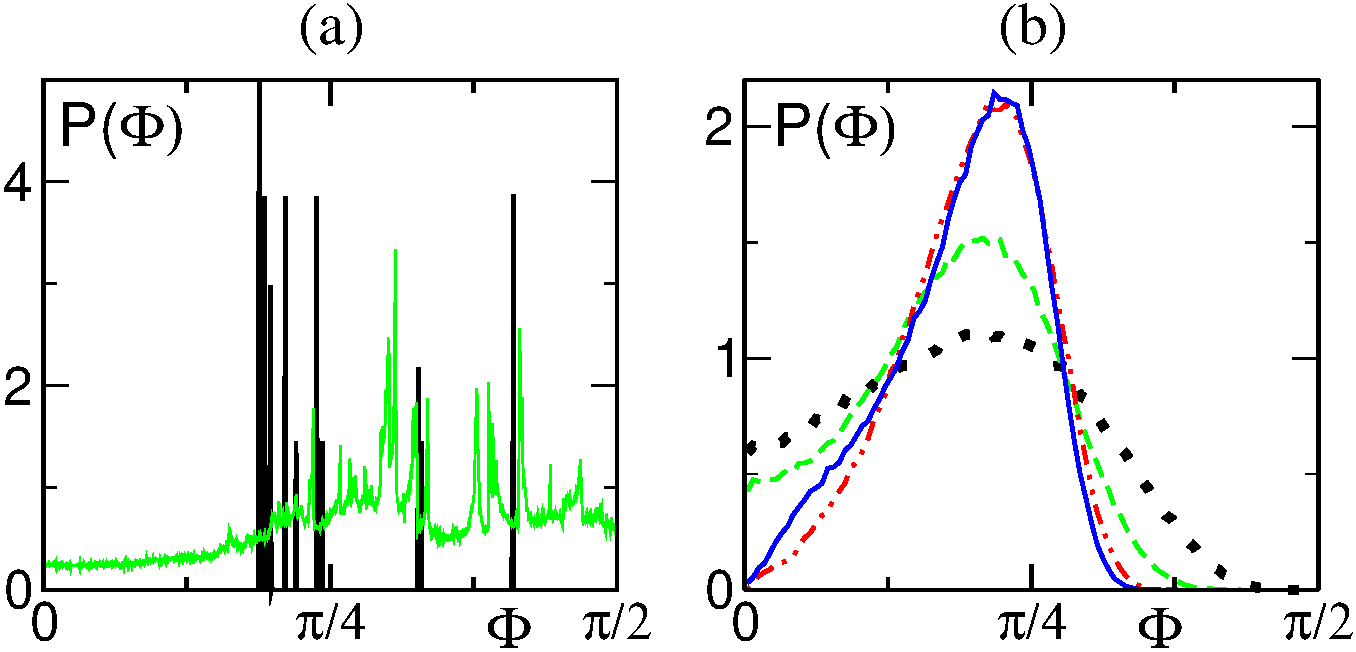
\includegraphics[width=0.85\textwidth]{gin99angle}
\end{center}
\caption{
(a) Probability distribution of the angle between stable and
unstable manifold for the H\'enon map $x_{n+1} = 1 -1.4\,
x_n^2 + 0.3 x_{n-1}$, and the Lozi map $x_{n+1} = 1
-1.4\,|x_n| + 0.3 x_{n-1}$ (black line, rescaled by a factor
10). (b) Ignore this frame.
}
\label{fig:gin99angle} %{Hyp}
\end{figure}
%%%%%%%%%%%%%%%%%%%%%%%%%%%%%%%%%%%%%%%%%%%%%%%%%%
%

A dynamical system is said to be \emph{hyperbolic} if its
\statesp\ has no homoclinic tangencies, \ie, the stable and
unstable manifolds are everywhere transversal to each other.
Since {\cLvs} correspond to the local
expanding/contracting directions, one can compute their
relative transversality and quantify the degree of hyperbolicity.
The knowledge of the {\cLvs} allows testing hyperbolicity by
determining the angle between each pair $(j,k)$ of expanding
($j$) and contracting ($k$) directions
\[
\phi_n^{j,k} = \cos^{-1}(|{\bf v}_n^{(j)} \cdot{\bf v}_n^k|) \in [0,\pi/2]
\,.
\]
As a test, Ginelli \etal\rf{ginelli-2007-99} compute the
probability distribution $P(\phi)$ of $\phi_n^{1,2}$ for the
H\'enon and Lozi two-dimensional maps. Arbitrarily small
angles are found for the H\'enon map, while the distribution
is bounded away from zero in the Lozi map \reffig{fig:gin99angle},
consistent with the Lozi map being hyperbolic\rf{CoLe84}.

\item[2011-02-26 Predrag]
{\em Covariant Lyapunov vectors for rigid disk systems}
by Hadrien Bosetti, Harald A. Posch\rf{BoPo10}. They say:

``We study the Lyapunov instability of a two-dimensional hard disk system
in a rectangular box with periodic boundary conditions. The system is
large enough to allow the formation of Lyapunov modes parallel to the $x$
axis of the box. The Oseledec splitting into covariant subspaces of the
tangent space is considered by computing the full set of covariant
perturbation vectors co-moving with the flow in tangent-space. These
vectors are shown to be transversal, but generally not orthogonal to each
other. Only the angle between {\cLvs} associated with immediate
adjacent Lyapunov exponents in the Lyapunov spectrum may become small,
but the probability of this angle to vanish approaches zero. The stable
and unstable manifolds are transverse to each other and the system is
hyperbolic.''

%
%%%%%%%%%%%%%%%%%%%%%%%%%%%%%%%%%%%%%%%%%%%%%%%%%%
\SFIG{BoPo10-Fig1small} {}{
The H\'enon attractor (black line) and a finite-length approximation of
its stable manifold (dotted line) are shown. The red vectors are the
{\cLvs} at the phase point 0 as explained in the main text. The
blue vectors are Gram-Schmidt vectors.
}{BoPo10-Fig1}
%%%%%%%%%%%%%%%%%%%%%%%%%%%%%%%%%%%%%%%%%%%%%%%%%%
%
I particularly like their H\'enon attractor illustration,
\reffig{BoPo10-Fig1}. [Might use their BoPo10-Fig1.eps in ChaosBook.org;
if so, ask for permission.]

\item[2011-07-08 Predrag]
Hiroki Takahasi, Miki U. Kobayashi, Kazuyuki Aihara,
\emph{How horseshoes are destroyed and what comes afterwards}:

``
We investigate the dynamics of strongly dissipative H\'enon maps at the
first bifurcation parameter at which the uniform hyperbolicity is
destroyed by the formation of tangencies inside the limit set. In a
parameter interval of transition from horseshoes to chaotic attractors,
we prove that the relative frequency of chaotic transient tends to one as
the Jacobian tends to zero. We also present numerical results which
support the conjecture of Lai Y-C, Grebogi C, Yorke J.A., Kan I (1993
Nonlinearity 6 779-797) on the frequency of non-hyperbolic chaotic
transient.
''

\item[2011-07-08 Predrag]
A mathematical paper, perhaps not directly relevant to the Lyapunov
project.
Hiroki Takahasi,
\emph{Prevalent dynamics at the first bifurcation of the H\'enon map},
\arXiv{1011.4200}:

``
We study the dynamics of strongly dissipative H\'enon maps, around the
first bifurcation parameter a* at which the uniform hyperbolicity is
destroyed by the formation of tangencies inside the limit set. We prove
that a* is a full Lebesgue density point of the set of parameters for
which Lebesgue almost every initial point diverges to infinity under
positive iteration. A key ingredient is that a* corresponds to
``non-recurrence of every critical point,'' reminiscent of Misiurewicz
parameters in one-dimensional dynamics. Adapting on the one hand
Benedicks-Carleson's parameter exclusion argument, we construct a set
of ``good parameters'' having a* as a full density point. Adapting
Benedicks-Viana's volume control argument on the other, we analyze
Lebesgue typical dynamics corresponding to these good parameters.
''

\item[2011-06-30 Predrag] \arXiv{1106.4929},
\emph{Simulating rare events in dynamical processes},
by Cristian Giardina, Jorge Kurchan, Vivien Lecomte,
and Julien Tailleur\rf{GiKuLeTa11}. They say:

``
Untypical, rare trajectories of dynamical systems are important: they are
often the paths for chemical reactions, the haven of (relative) stability
of planetary systems, the rogue waves that are detected in oil platforms,
the structures that are responsible for intermittency in a turbulent
liquid, the active regions that allow a supercooled liquid to flow...
Simulating them in an efficient, accelerated way, is in fact quite
simple.
''

This method is of interest to us because I suspect that the
`nonhyperbolicities' that Ginelli\etal\rf{YaTaGiChRa08} find are
localized to a few tangencies in the \statesp. They do not see this,
because they just compute without looking at the attractor, but for
example I expect this will be very clear if one takes a look at the
H\'enon attractor. The flat distribution in stable/unstable angles arise
presumably {\em only} from close passage to the 13-cycle nearly tangent
periodic point discussed in Artuso and Aurell and
Cvitanovi{\'{c}}\rf{AACII} and in ChaosBook version 13 (see exercise
17.1. ``How unstable is the H\'enon attractor?''; sect. 29.1 ``Fictitious
time relaxation''; Table 29.1).

\item[2011-08-25 Hugues]
Kazz and I have decided to try a number of things, including looking at
H\'enon and the famous period-13 orbit. We will first calculate the CLV
along the orbit, to see how "non-hyperbolic" it is, and then extract from
the chaotic trajectory near-tangencies, and compare their location to the
period-13 orbit. {\bf 2011-10-02 Predrag} This discussion is continued on
\refpage{fig:HenonNonHypPoints}.

\item[2011-06-30 Predrag 2 Kazz]
I suspect that the  non-hyperbolicities that
Ginelli\etal\rf{YaTaGiChRa08} find are localized to a few tangencies in
the \statesp. They do not see this, because they just compute without
looking at the attractor, but for example I expect this will be very
clear if one takes a look at the H\'enon attractor. The flat distribution
in stable/unstable angles arise presumably {\em only} from close passage
to the 13-cycle nearly tangent periodic point discussed in Artuso and
Aurell and Cvitanovi{\'{c}}\rf{AACII} and in ChaosBook version 13 (see
exercise 17.1. ``How unstable is the H\'enon attractor?''; sect. 29.1
``Fictitious time relaxation''; Table 29.1).

Kazz, can you color code the small angles while running your code on the
H\'enon attractor? Maybe the 13-cycle will just jump out...

\item[2011-10-02 Kazz]
Here is the first data on the H\'enon map.
\refFig{fig:HenonNonHypPoints}\,(a) shows the angle between the two
Floquet eigenvectors (computed as CLVs) of three \po s, one is hyperbolic
and the others are (almost) non-hyperbolic. Specifically, the former is
the third $\cl{}=10$ orbit $p_{10c} = \cycle{0011111101}$, and the latter
the two $\cl{}=13$ orbits $p_{13a} = \cycle{1110011101000}$ and $p_{13b}
= \cycle{1110011101001}$ in Table 29.1 in
\HREF{http://chaosbook.org/version13/paper.shtml\#relax}{Chaosbook.org},
p.~564, here reproduced as \reftab{t-biham2}. For notation, see
\refappe{s-SymbDynDefs}.

The angle is shown as a function of time over one period. As you
see, while the angle for the hyperbolic orbit is at least 0.4 (i.e.,
indeed hyperbolic), the angle for the $p_{13a}$, $p_{13b}$ orbits reaches 0.04
at $t=11$ (indeed almost non-hyperbolic).

% PC 2011-10-02: generated by Kazz
\begin{figure}
 (a)~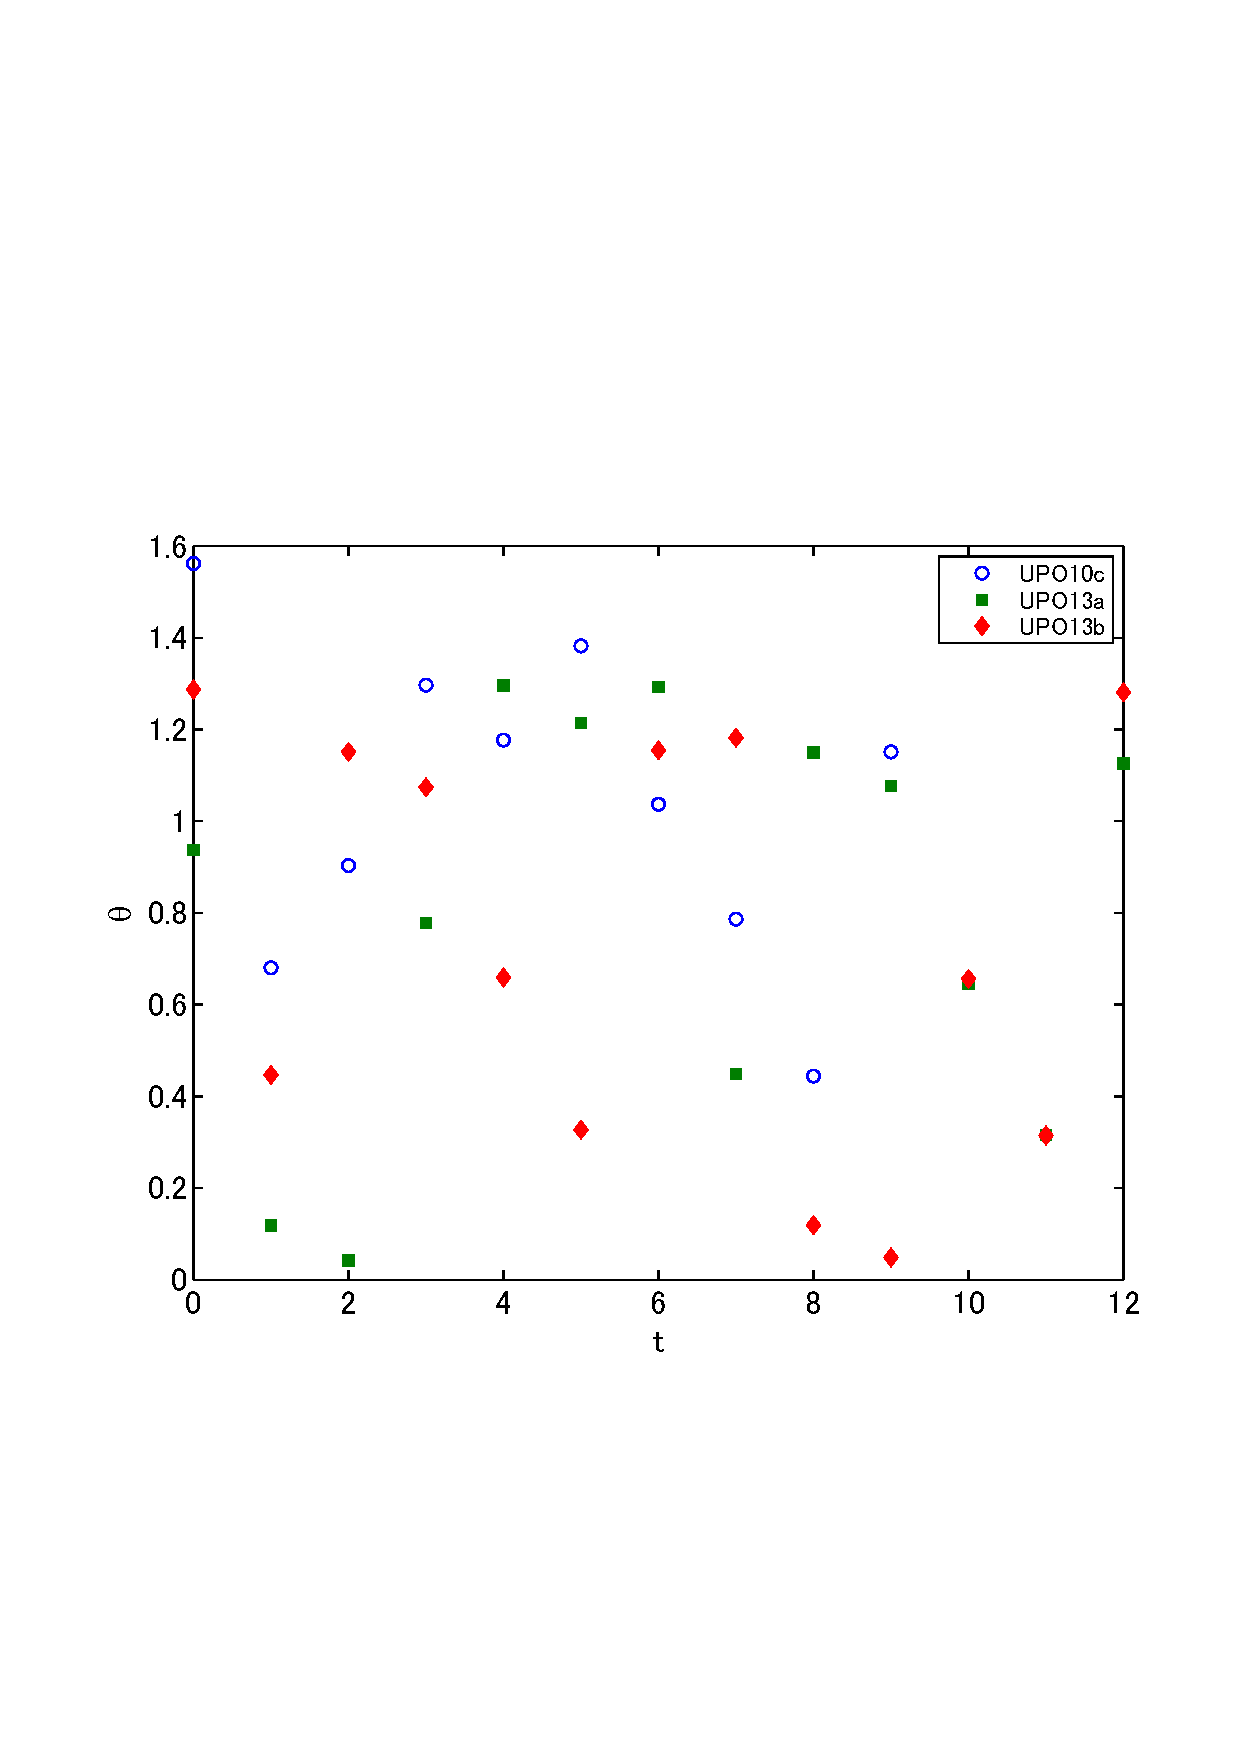
\includegraphics[width=0.45\textwidth]{fig1-hyperbolicity}
 (b)~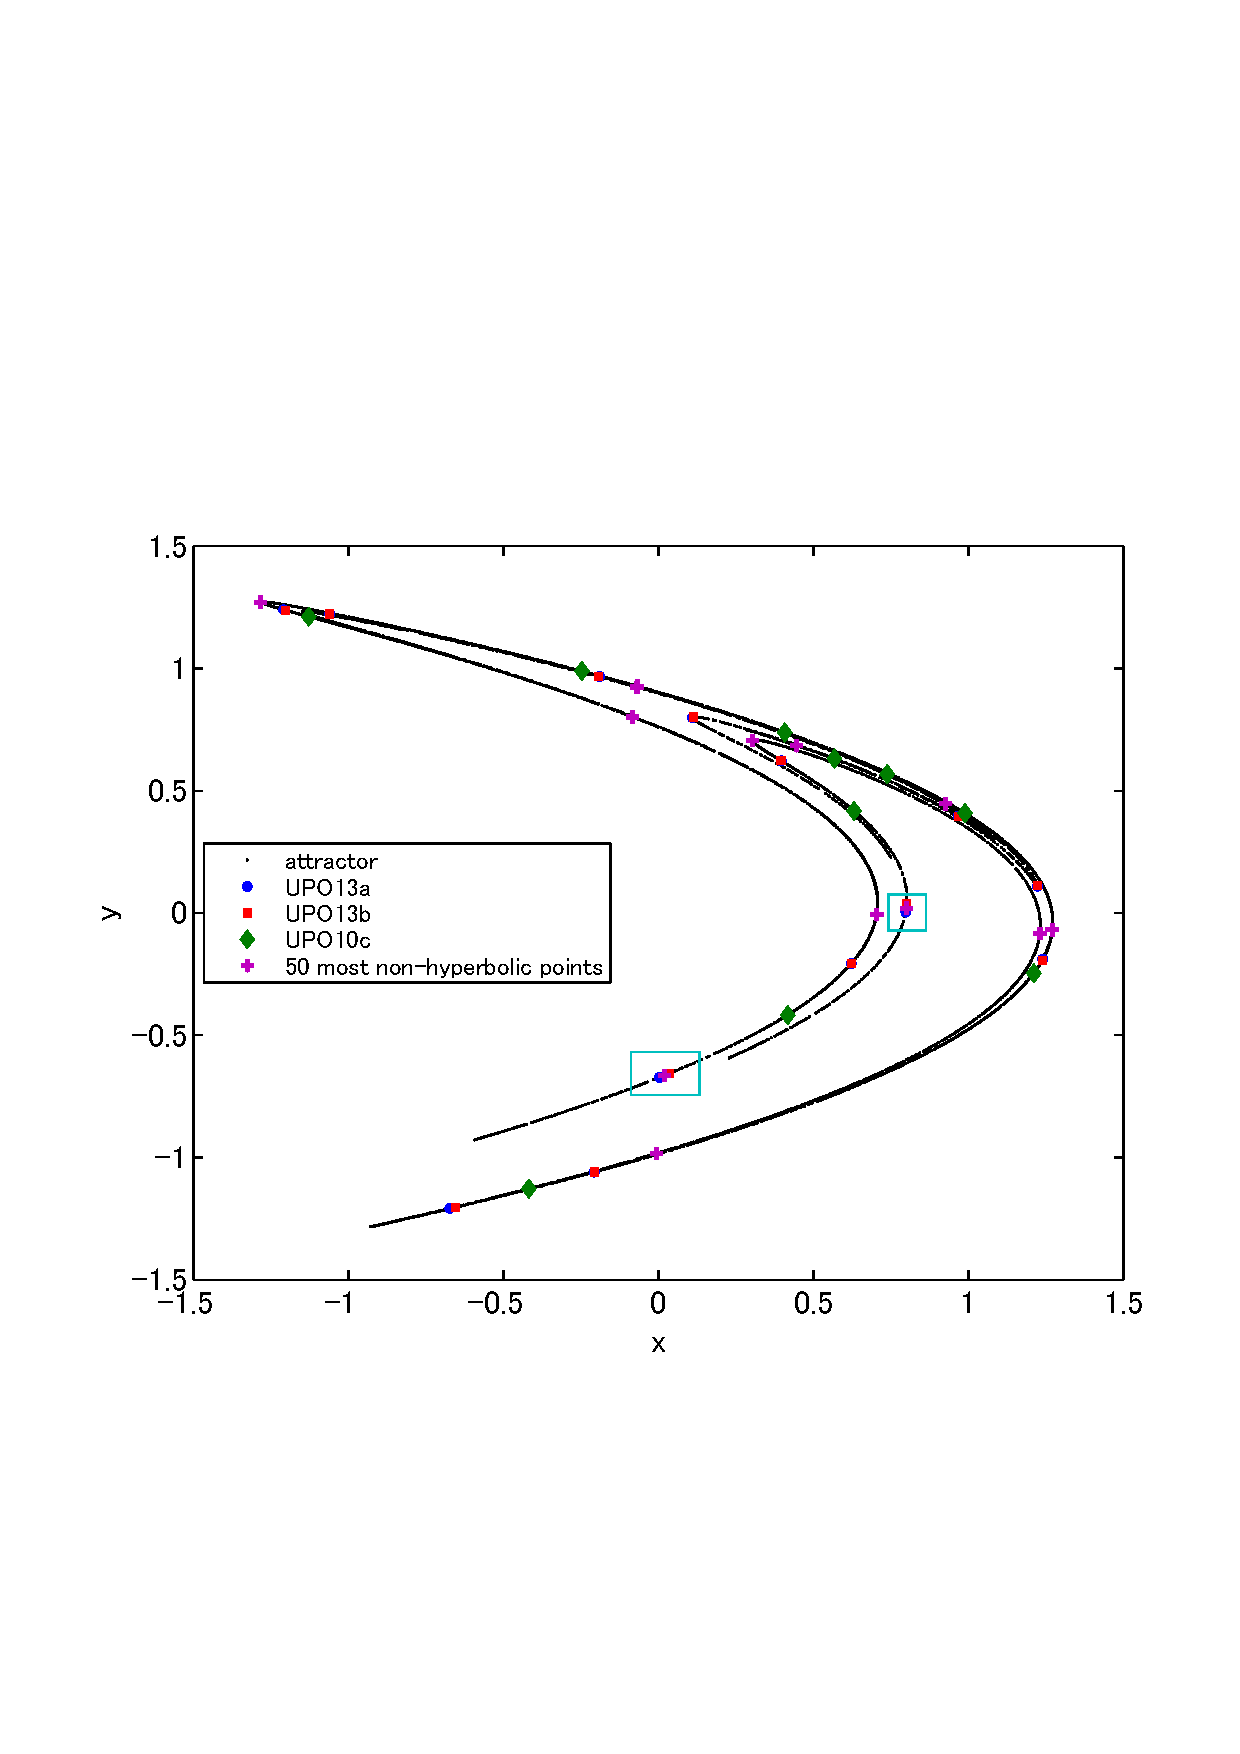
\includegraphics[width=0.45\textwidth]{fig2-nonhyp_points}
\caption{
(a)
(b)
[Kazz 2011-10-02].
}
\label{fig:HenonNonHypPoints}
\end{figure}

Here I use improved initial conditions for the \po s and the results did
not change.

\refFig{fig:HenonNonHypPoints}\,(b) shows, on the top of the H\'enon attractor,
all the points of the above three \po s (filled symbols, not the same ones
as \reffig{fig:HenonNonHypPoints}\,(a)) as well as the 50 most non-hyperbolic
points along a chaotic trajectory of length $10^6$ (plus symbols; most
non-hyperbolic means smallest angle here). We see that some of these
non-hyperbolic points are found very close to the non-hyperbolic \po s
(see inside the light blue rectangles), while none of the non-hyperbolic
points are close to the hyperbolic \po. However, we see that many
non-hyperbolic points are actually far enough from the two non-hyperbolic
\po s, suggesting that there are other non-hyperbolic \po s in this system.

\item[2011-10-03 Predrag] I do not remember other cycles being as
non-hyperbolic as these 13-cycles, but I should have a database of
thousands (?) of  H\'enon cycles somewhere, if you want to have a look...

\item[2011-10-06 Predrag]
Have a look at {\bf 2011-07-01 Predrag} post on Greene and Kim\rf{GreeKim87}
in \refchap{s:LyapunovVec}.

\begin{figure}
(a)
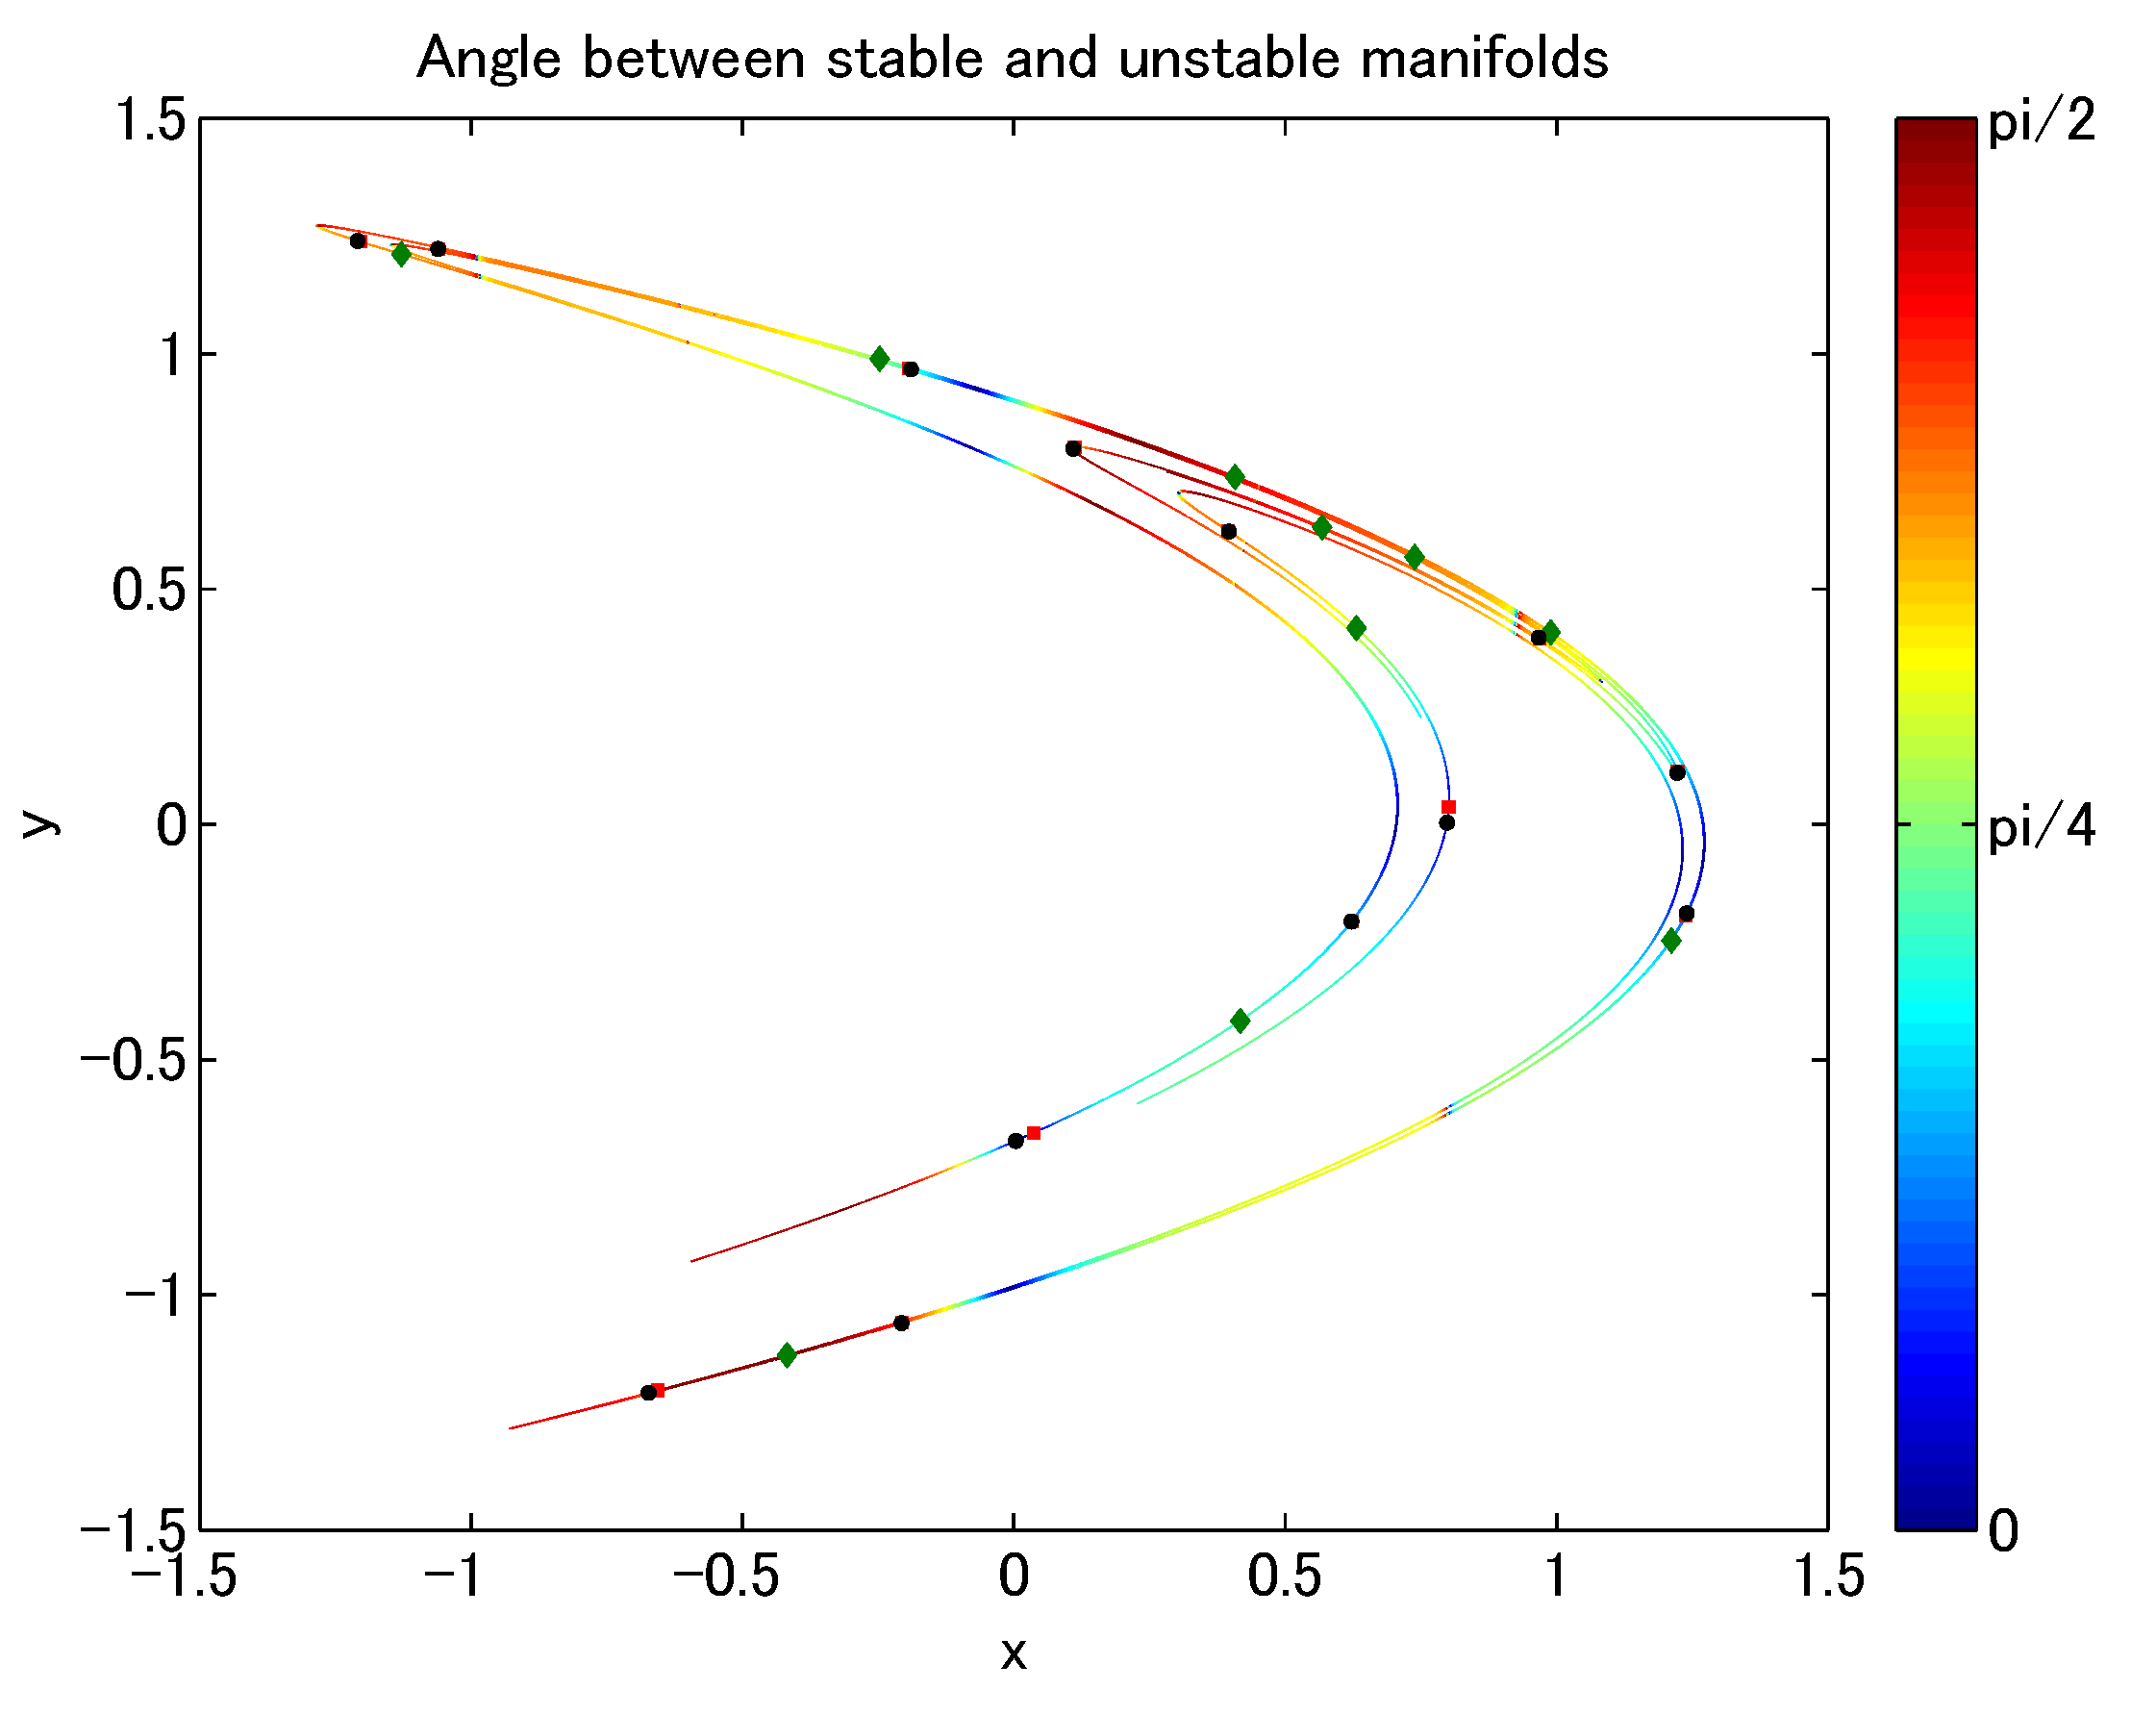
\includegraphics[width=0.45\textwidth]{fig3-angle}{}
(b)
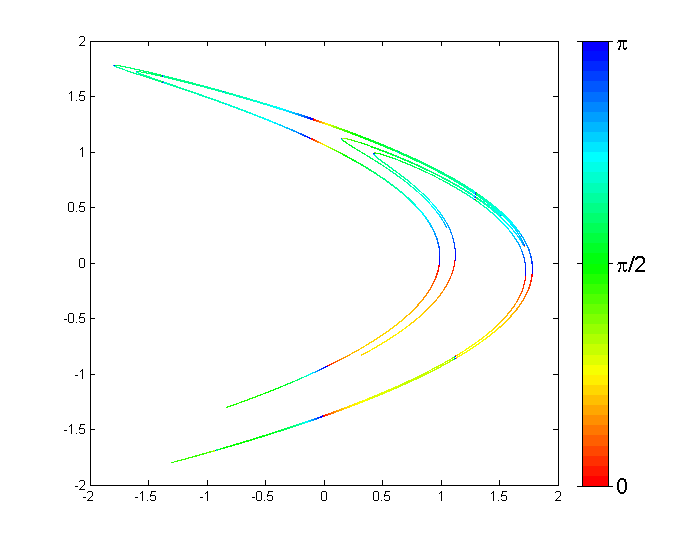
\includegraphics[width=0.45\textwidth]{henon_su_angle}{}
\caption{
(a)
The relation between the non-hyperbolicity of the chaotic trajectory and
\po s. The color code indicates the angle between the stable and unstable
manifolds, and the symbols are the positions of \po s (black circles =
$p_{13a}$, non-hyperbolic; red squares = $p_{13b}$, non-hyperbolic; green
diamonds = $p_{10c}$, hyperbolic). It shows that the degree of the
non-hyperbolicity is a smooth function along the attractor, and around
the most non-hyperbolic point of  $p_{13a}$, $p_{13b}$ (near (0.8,0)) the
chaotic trajectory is also non-hyperbolic. The figure also shows that
there are other non-hyperbolic \po s that are not found, because there
are blue regions close to none of the cycle points of $p_{13a}$,
$p_{13b}$ \po s. (click
\HREF{https://www.sugarsync.com/pf/D6368502_0823551_99453}{here} for the
humongous original.)
(b)
Homoclinic tangencies are places where the angle changes from $0$ to
$\pi$.
    }
\label{fig3-angle}
\end{figure}


% PC 2011-10-06: generated by Kazz
\begin{figure}
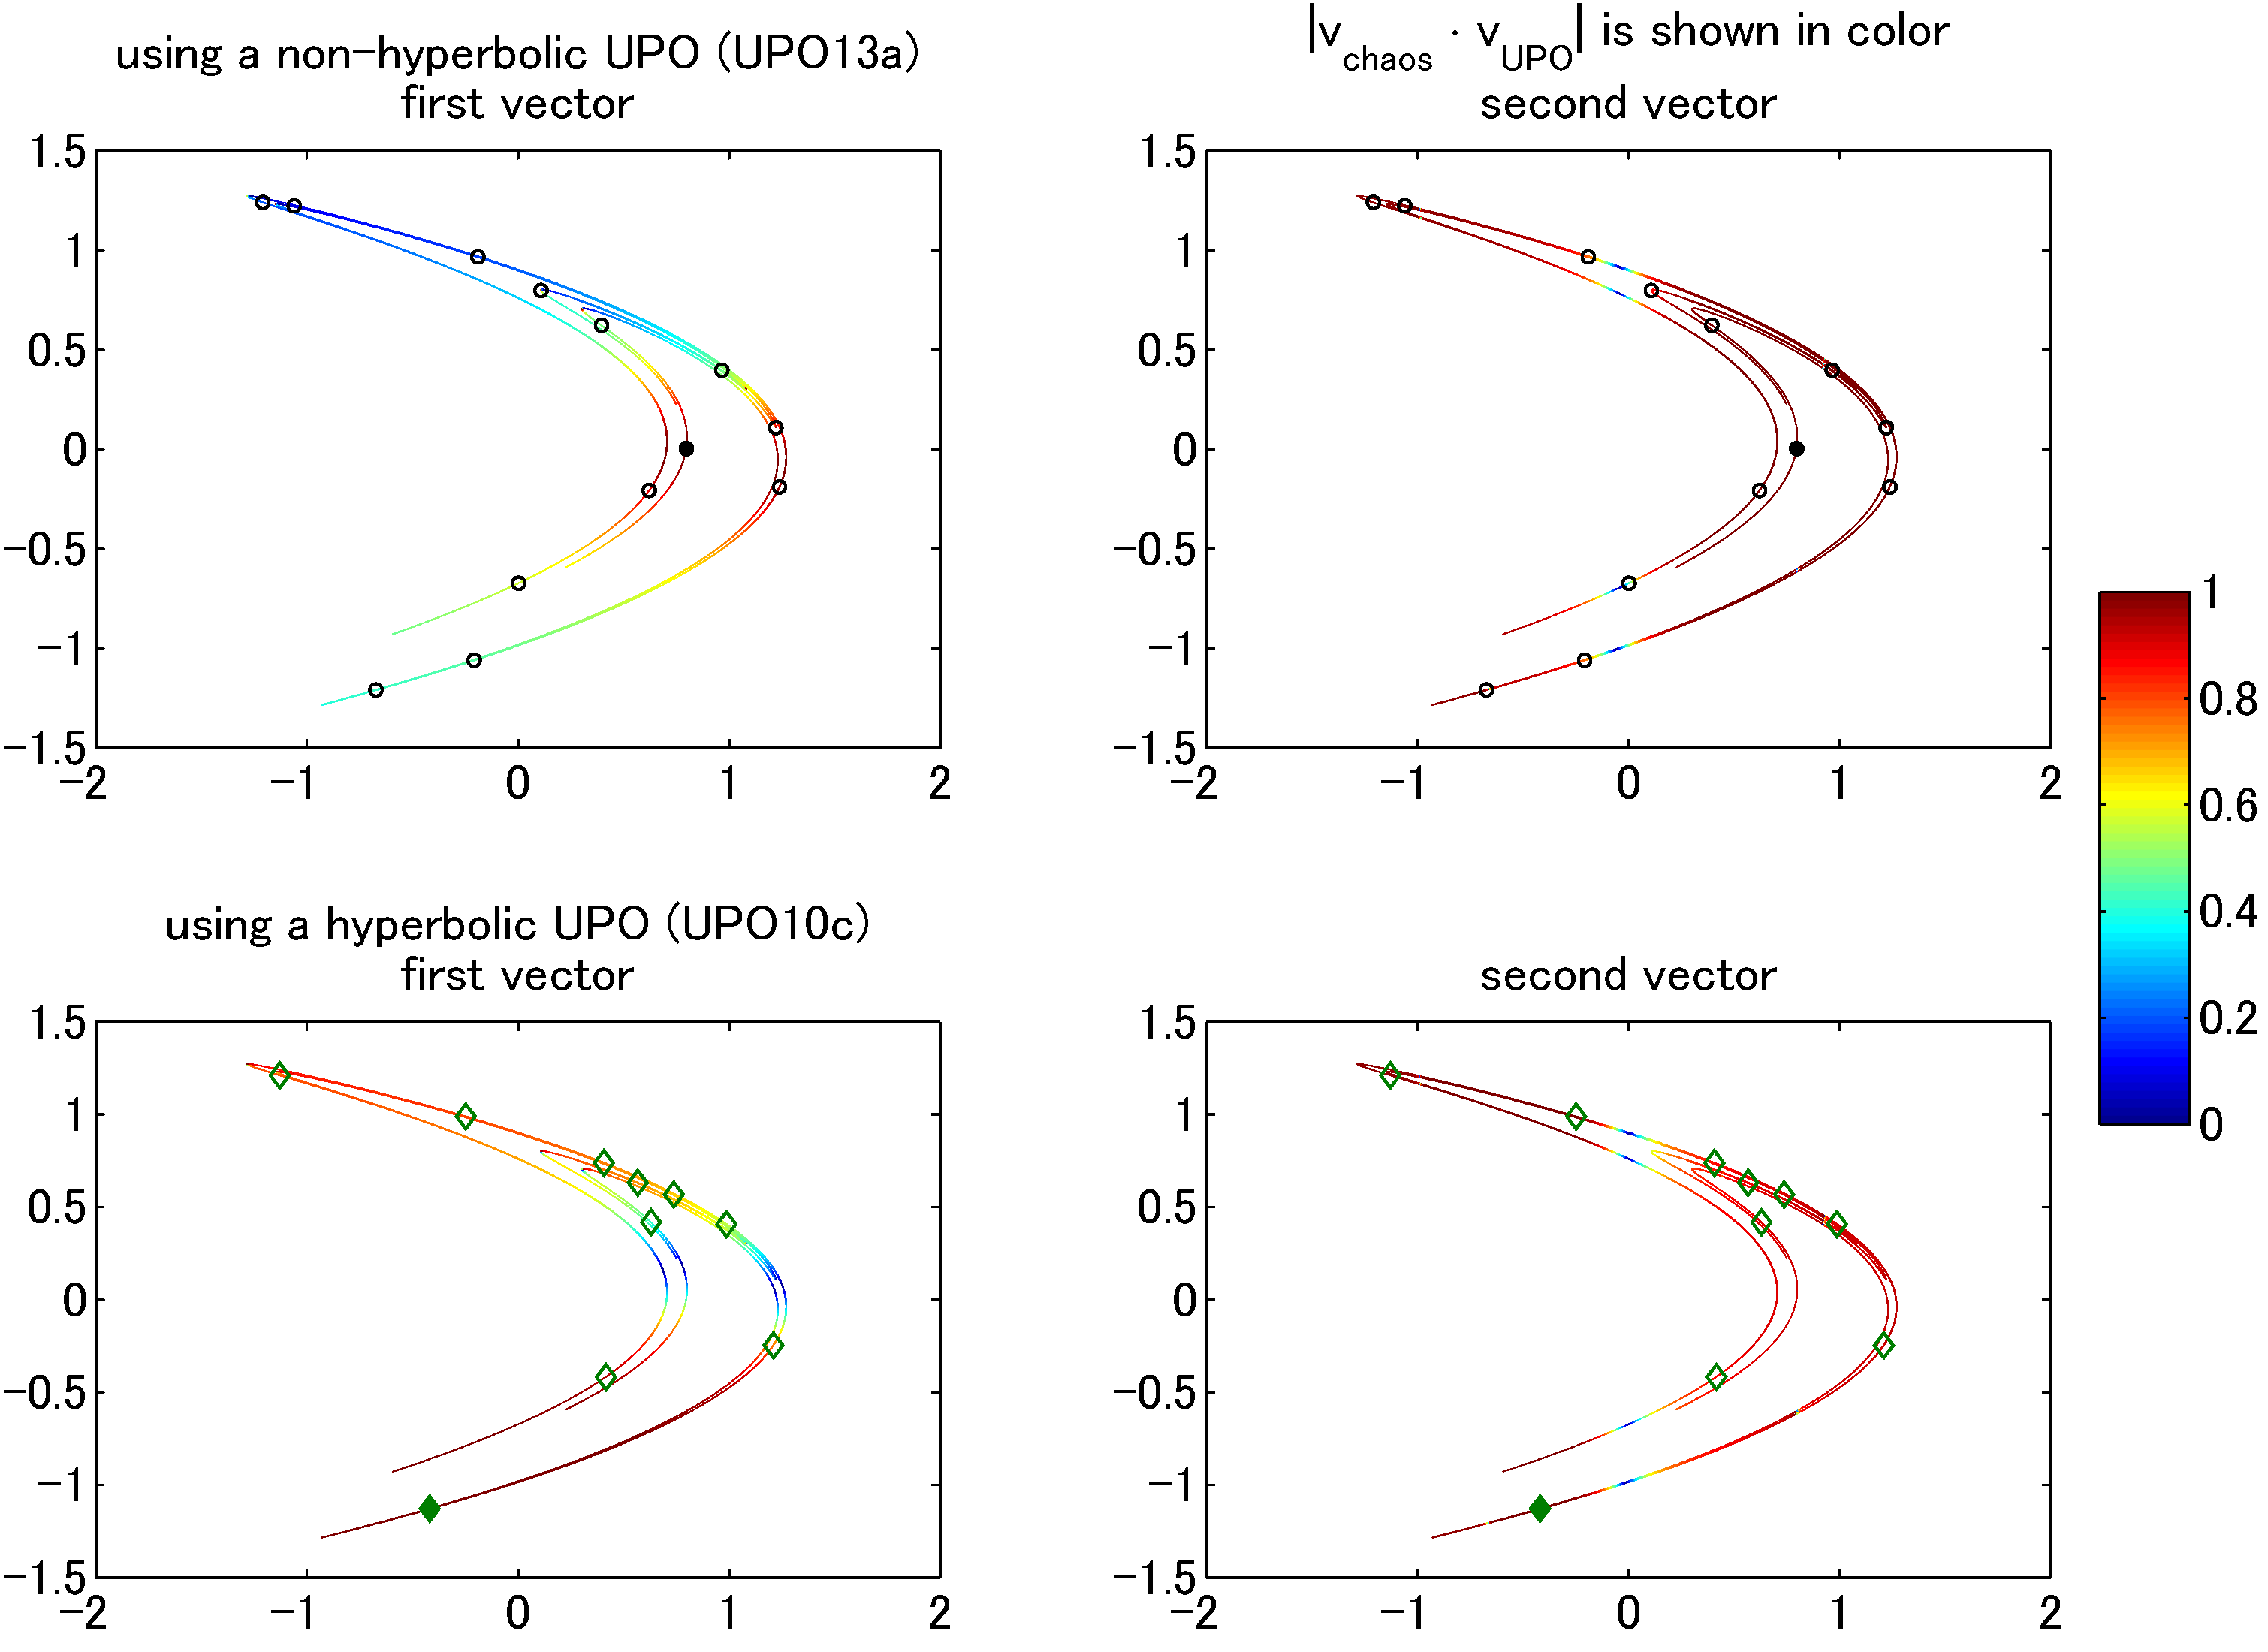
\includegraphics[width=0.95\textwidth]{fig4-VectorSimilarity}
\caption{
The similarity between the first (second) Lyapunov vectors of the
chaotic trajectory and an \po\ ($p_{13a}$ or $p_{10c}$). Specifically, the color
code indicates the absolute value of the dot product of the two vectors
to compare. Here, I choose one point of the \po s (most non-hyperbolic
point for $p_{13a}$ and most hyperbolic point for $p_{10c}$; shown by filled
symbols) and compare a \po\ vector of that point with the vector of the
chaotic trajectory at all the points along the trajectory. You see that
the two vectors are quite similar if the chaotic trajectory is close to
the reference point (filled symbol), regardless of the index and the
hyperbolicity of the \po s.
(click \HREF{https://www.sugarsync.com/pf/D6368502_0823551_99467}{here} for
the humongous original)
}
\label{fig4-VectorSimilarity}
\end{figure}


\item[2011-10-06 Kazz]
New, improved \reffig{fig3-angle}\,(a) and \reffig{fig4-VectorSimilarity}.

\item[2011-10-06 Hugues]
It seems pretty clear to me that there exists (infinitely) many "almost
non-hyperbolic" \po s and all the more so than they have longer periods
(remember the plots "minimum angle vs period" of Kobayashi and Saiki).
But, now, how to find them? Would starting points given by points at
which the CLVs of the chaotic trajectory are almost tangent be useful?

\item[2011-10-06 Kazz]
There should be many \po s flowing like the chaotic trajectory. They
therefore have long periods and are non-hyperbolic (almost, always). But,
in my view, it would be interesting to decompose properties of the
chaotic trajectory into those of only a few number of \po s, whose period
is rather short and thus each of which covers only a local region of the
attractor. For the H\'enon map, we are still lacking such a minimal \po,
which accounts for the remaining non-hyperbolic points of the chaotic
trajectory.

\item[2011-10-06 Predrag]
Wow! This comment makes no sense, but it does smack of the famous
Japanese Heresy that Evangelos can explain. There is NO such thing -
instead of this there is perfectly well developed theory that says how
you use \po s and how many do you need to capture the hyperbolic parts of
the {\nws}. It's as elegant and systematic as Stat Mech and Quantum Field
Theory. Read \HREF{http://chaosbook.org/}{The Book}. But who reads books
nowadays? BTW, there is no need to attach prefix U to \po s; there are a
few or no stable orbits in chaotic dynamics, and exponentially many
unstable ones, it's some dumb Soviet style abbreviation that must have
come from Maryland or somewhere.

\item[2011-10-06 Predrag]
Yes, we used to call forward images of the primary H\'enon tangencies
`turnbacks' and such. My theory of
\HREF{http://www.cns.gatech.edu/~predrag/papers/preprints.html\#GeomChaos}{pruning
fronts} says that you only have to identify non-hyperbolicities on the
pruning front, the rest are just forward/backward images of it, and I
like to do it best by sequences of periodic orbits. Grassberger likes to
do it it by stable/unstable manifolds, but I hope that by now you agree
with me that the cycles are the way to go. The brilliant thing about the
pruning front is that you search for non-hyperbolicities systematically,
on a (fractal) line, rather than in the whole plane. This way you
systematically obtain the grammar of admissible itineraries for the
H\'enon-type maps. There are infinitely many nearly non-hyperbolic
cycles, but in practice at most one pair for each time step in the
period. The moment you find \emph{one} cycle that is stable, you have
proven that the H\'enon attractor is not a strange attractor, but rather
a strange repeller: there is roughly 50-50 chance that it is strange /
not strange for \emph{the} H\'enon parameter values. The moment
Grassberger heard my seminar he was able to compute all cycles up to
length 32 or so. Procaccia misunderstood what it was about and just
published it\rf{pre88top}, using partially my notes and adding 1/2
Procaccian gibberish to it, so that pretty much killed the joy of writing
it up for me, it has never been written up well. An attempt is in
\HREF{http://chaosbook.org/paper.shtml\#smale}{ChaosBook.org} chapter
{\em Stretch, fold, prune}.

\item[2011-10-07 Ruslan] Maybe this is not very relevant to your
discussion, but the angle between stable and unstable manifolds in 2-D
maps varies between $0$ and $\pi$.  The pictures should look something
like \reffig{fig3-angle}\,(b).

Anyway, some time ago I have been looking at H\'enon and Ikeda
maps trying to identify 'primary' tangencies, but couldn't do it
for the latter based on the manifolds (a la Grassberger). Predrag,
are you saying that non-hyperbolicities on the pruning front
uniquely define primary tangencies?  If yes, then I better go read
this chapter...

\item[2011-10-06 Hugues]
About the apparent smoothness of the angle between stable and unstable
manifolds: can't this information already be seen using (finite-length)
approximations of the stable manifold, as in Posch et al, Fig~3.4 of the
Blog? It seems to me that one can infer from such data how the angle
varies all along the attractor (following a sheet) and in particular one
should be able to locate the main (near-)tangencies with good accuracy.

\item[2011-10-07 Ruslan] In fact, a good approximation to the angle can
be found not just on the attractor, but extended across the whole plane
by looking at the most contracting directions of the Jacobian matrix of
the iterated forward and inverse maps.  This was done by Jaeger and Kantz
algorithm\rf{jaeger_kantz}, see \reffig{fig:henon_su_angle_plane}.

\begin{figure}
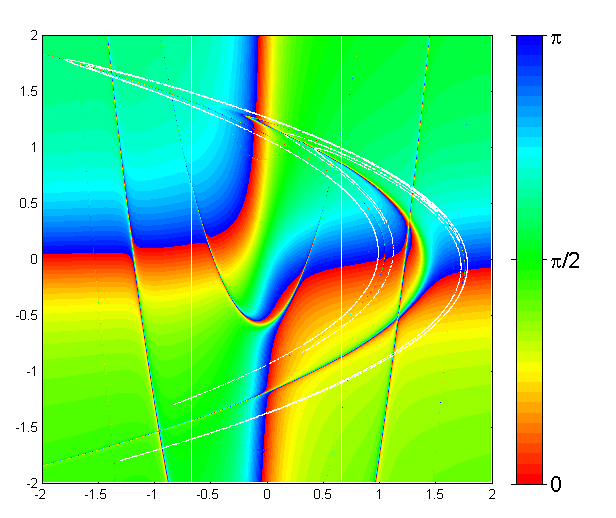
\includegraphics[width=0.95\textwidth]{henon_su_angle_plane}
\caption{
A finite time, color coded approximation to the most contracting
direction of the Jacobian matrix, iterated forward and inverse
maps, here seven iterates each way.
}
\label{fig:henon_su_angle_plane}
\end{figure}

\begin{figure}
(a)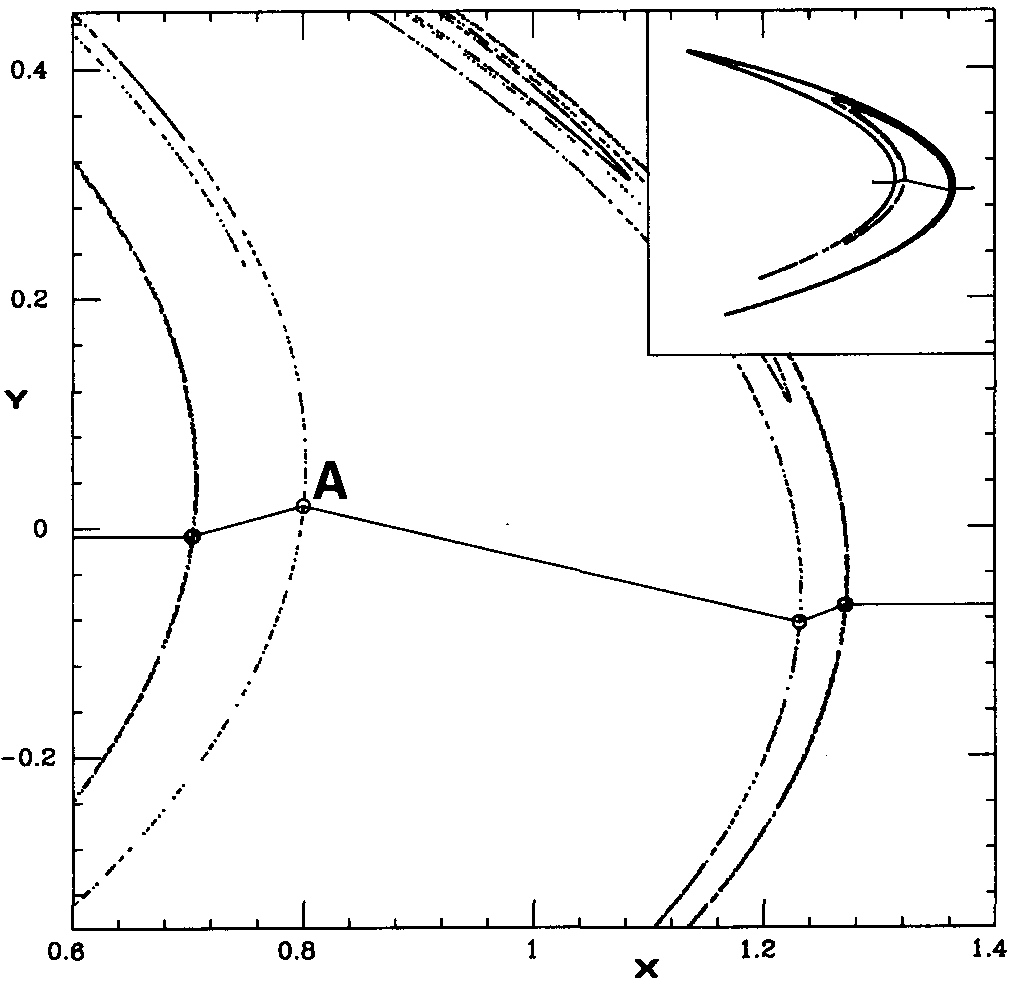
\includegraphics[width=0.47\textwidth]{fig1-AGIP90}
(b)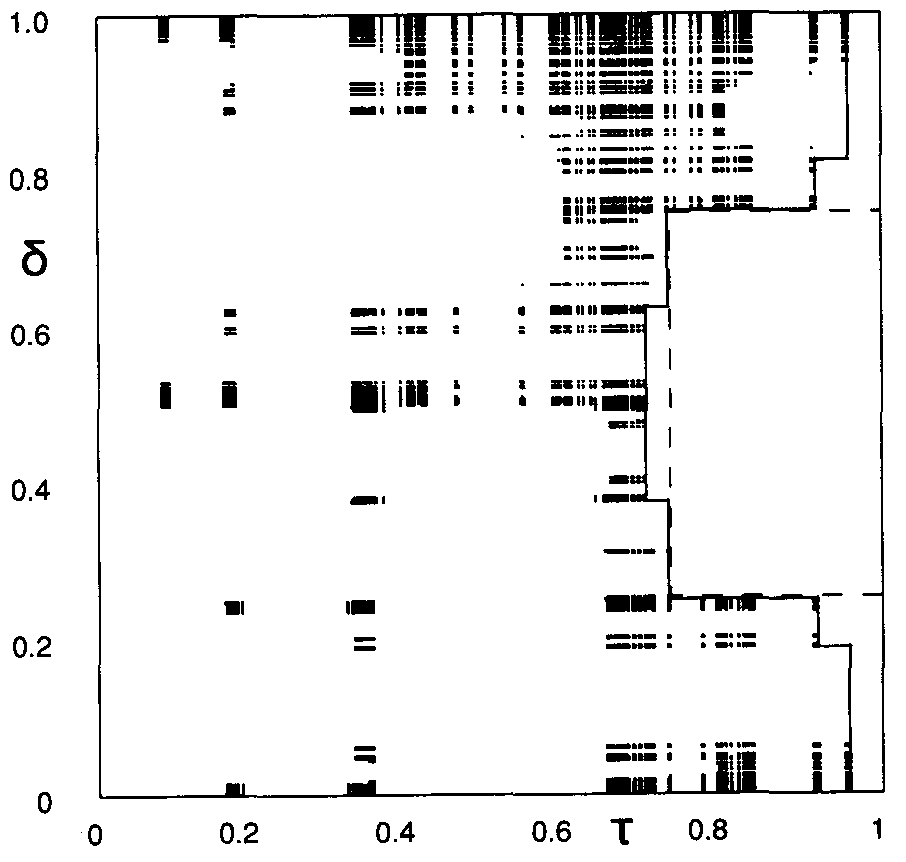
\includegraphics[width=0.47\textwidth]{fig2-AGIP90}
\caption{
(a)
The binary partition of the H\'enon attractor. The circles represent
altogether 500 primary homoclinic tangencies. The entire H\'enon
attractor is shown in the inset.
(b)
The symbol $(\tau,\delta)$ plane of the H\'enon map for $(a, b) = (1.4,
0.3)$. The pruning front is drawn as a full line. The broken line
represents the rectangle cut out by the tangency point '$A$' in (a).
(From \refref{AGIP90})
}
\label{fig1-2-AGIP90}
\end{figure}

\item[2011-10-08 Predrag 2 Ruslan] Thanks for arising from the dead, with
beautiful artwork, as always. Maybe I can keep you focused this time, as
it does deal with the sins of your youth. It has been Maryland religion
not to cite my work, which is bit inconsiderate, considering that their
zillion \po\ (or ``UPO'') papers started the moment Grebogi returned from
a conference in Israel in 1985? 1987? where he heard me explain how the
pruning front and zeta functions work in terms of \po s. On the other
hand, I just assumed (probably correctly - I know it first hand from
collaborating with Ott) that they did not understand it. Grassberger and
Kantz\rf{GK85}, however is a key contribution, and Peter understood
what it was about the moment I explained why I use Manhattan map of the
H\'enon, rather than its $(\ssp_n,\ssp_{n+1})$ embedding. Grassberger's
construction is equivalent to my theory of the H\'enon map symbolic
dynamics, the difference being only the long term goal of where are you
going with this thing. They visualize the `partition line' in
$(\ssp_n,\ssp_{n+1})$ coordinates, \reffig{fig1-2-AGIP90}\,(a), as they
think about the problem like you do, in terms of homoclinic tangencies,
\reffig{fig:henon_su_angle_plane}.

Click
\HREF{http://chaosbook.org/library/AGIP90.pdf}{here} for \refref{AGIP90}.
Some nice figures, very well written, worth a look.
They write: ``
Our final conclusion is that both the Grassberger and Kantz\rf{GK85}
generating partition, and the Cvitanovi\'c \etal\rf{pre88top} pruning
front have passed extremely precise numerical tests. Also the ideas put
forward in \refref{DAlesPol90} were verified substantially. The most
precise understanding of the topological dynamics was not through
\po s, but by directly studying the homoclinic tangency points
defining the pruning front. Once this is understood, the transition to a
description in terms of \po s is possible and interesting.''

\item[2011-10-09 Predrag]
I want to take the construction to arbitrarily high dimension, where
there is no way to plot \reffig{fig:henon_su_angle_plane}, or the
homoclinic tangencies, and therefore I pin down the non-hyperbolicities
(primary folds of the attractor) by bracketing them between pairs of \po
s whose symbolic dynamics we understand better and better the longer our
cycles are (and variational methods enable us to compute cycles of
arbitrary length: 1\,000, 10\,000, whatever we need, as long as it is
only one cycle of fixed itinerary rather than all $2^{10\,000}/10\,000$
prime cycles. The beauty of the partition line is that you immediately
grasp that there are \emph{very few} non-hyperbolic \po s - a small
fractal dimension (the dimension of the attractor in the stable manifold
direction) more than just one pair per each cycle length. The beauty of
the pruning front, \reffig{fig1-2-AGIP90}\,(b), is that it predicts the
symbolic sequence for the next pair of cycle points on each fold, so you
can go far. While the partition line would require figuring out the
embedding of \KS\ 10-20\dmn\ stable / unstable physical manifolds in
1\,000\dmn\ \statesp, the pruning front is constructed by computing
systematically sequences of \po s.

Our first triumph was killing\rf{DR_prl} what until then was one of the
few physical potentials believed to be fully ergodic, the $x^{2}y^{2}$
potential: the elliptic island's area is -let's say- $\approx 10^{-13}$, so you
would never find it by starting random trajectories, you can only do it
by  resolving systematically the pruning front. It has not been seriously
attempted for the H\'enon attractor - that is a big gamble, as unless you
find a stable cycle you have not disproved ergodicity, and it is a
50-50\%\ crap shoot whether it is ergodic or not for precise
parameters values H\'enon used. However, Lan\rf{lanCvit07} was able to find a
very long attractive (but looking chaotic) cycle in \KS\ by a very crude
version of such search, which also would be unthinkable if you were
scanning the \statesp\ (the orbit is at least 60 times longer than the
shortest cycle, and its immediate basin of attraction is very small).

\item[2011-10-06 Kazz]
Given that the CLVs are local linear approximations for the unstable and
stable manifolds and assuming that these manifolds do not depend on the
position on the chaotic attractor, this should provide the same
information as the angle between the CLVs. Then I think it's easier to
compute the CLV angle directly.

\item[2011-10-06 Predrag]
Bit more subtle than that - turnbacks on long cycles are very sharp and
very small, so things that look smooth are not smooth; they are dense,
and everyplace on the strange attractor. Turnbacks are visible as
singularities in natural measure (that's always a signature of
non-hyperbolicity, see Figure~16.6 in
\HREF{http://chaosbook.org/paper.shtml\#measure}{ChaosBook.org} chapter
{\em Transporting densities}. The good news is the pruning front theory:
you need to only identify (near-)tangencies on the smooth primary folds,
all the sick stuff then comes for free, by iterating the cycles that
bracket the tangency.

\item[2011-10-06 Kazz]
I have no experience of finding \po s, but I'm sure starting from
non-hyperbolic points is useful. The most primitive way for discrete-time
systems like H\'enon would be simply trying the Newton method for
arbitrarily chosen periods. If it converges to a point near-by, we get
it!

\item[2011-10-06 Predrag]
It's a solved problem - you read chapter
\HREF{http://chaosbook.org/paper.shtml\#cycles}{Fixed points, and how to
get them} first, implement it to get short cycles (or ask Evangelos to
hand you the code), and then you read chapter
\HREF{http://chaosbook.org/paper.shtml\#relax}{Relaxation for cyclists}
to learn how to find ALL cycles up to a given topological length, (or ask
Lan to hand you the code). Hyperbolic cycles are easy - the pain are the
non-hyperbolic ones, that's explained in chapter
\HREF{http://chaosbook.org/paper.shtml\#inter}{Intermittency}, but I do
not think this is useful to us at this point.

\item[2011-10-06 Kazz]
by the way I noticed that the definition of the H\'enon map in ChaosBook
\bea
    x_{n+1}&=&1-ax^2_n+b y_n
        \continue
    y_{n+1}&=& x_n
\label{eq2.1c}
\eea
is different from the ``standard'' one
\bea
    x_{n+1}&=&a - x_n^2 + b y_n
        \continue
    y_{n+1}&=& x_n
\label{eq2.1b}
\eea
but the used parameter values are the same ($a=1.4$, $b=0.3$). I didn't
realize it when I made my code and used ChaosBook's definition. I'd like
to know if you really used the former definition to obtain \po s, for
example, and if the nature of chaos does not change for both definitions.

This is why the shape and the position of the attractor is different
(compare the coordinates of the attractor in my figure and that of
Posch).

\item[2011-10-06 Predrag]
The standard definition is surely H\'enon\rf{henon} own \refeq{eq2.1a}.
Some people chose to rewrite it as \refeq{eq2.1b}, as that is closer to
Fateau' quadratic polynomial, but there is no persuasive reason to mess
with H\'enon's definition, and I find it disrespectful. I even had a bad
experience with that kind of nonsense myself. Some mathematicians
experienced discomfort when period doubling universality was discovered.
When they finally worked it out, did exaaactly what Feigenbaum and I did
to solve the equation and the light went on, convergence of our Newton
iteration became a ``theorem'', they permuted several Greek letters and
signs on my period-doubling universal equation, and since then they
attach names of random mathematicians to it. Not nice.

\item[2011-07-24 Predrag]
                                    \toCB
You might find Demidov's website\rf{DemChaos} helpful, his simulations
are instructive. He uses a different definition for parameters $a$ and
$b$ from H\'enon, but unfortunately uses the same letters. Now, that's in
a really bad taste. His definition is natural if one is interested in
Julia sets, but unfortunately is not the one H\'enon used, and I always
try to follow the foundational papers, rather than confusing everybody
with unnecessary parameter redefinitions. Demidov\rf{DemChaos}
non-H\'enon  parametrization is
\bea
    x_{n+1}' &=& a'+ {x'}{}^2_n + b' y_n'
        \continue
    y_{n+1}' &=& x_n'
\,.
\label{DemidHen1}
\eea
(Note yet another screwy sign difference from the H\'enon convention)
Dividing through by $a'$ we get
\(
\frac{x_{n+1}'}{a'} = 1 + a'\left(\frac{x_n'}{a'}\right)^2 + b'\frac{y_n'}{a'}
\,,
\)
so the two parametrizations are related by:
\beq
x={x'}/{a'}
\,,\quad
y={y'}/{a'}
\,;\qquad
a=-{a'}
\,,\quad b= {b'}
\,.
\ee{DemidHenPar1}
After a while the light goes on, and you realize that H\'enon was
thinking: in his convention unit square remains unit square, with $a$
telling you how stretched the horseshoe is, and $b$ how compressed it is.
In some other random convention the frame of the map scales with $a$,
which is stupid. Please do me a favor, and do it as in ChaosBook. I've
worked on H\'enon-type maps for years, and there is no reason not to use
the consistent, established notation.

%%%%%%%%%%%%%%%%%%%%%%%%%%%%%%%%%%%%%%%%%%%%%%%%%%%%%%%%%%%%%%%%%%
\SFIG{Demidov_a-6_b-1}
{}{
PC: The Smale backward-forward horseshoe generated by the
Demidov\rf{DemChaos} java applets for the H\'enon parameter values
$(a,b) = (6,-1)$.
    }{Fig:Demidov1}
%%%%%%%%%%%%%%%%%%%%%%%%%%%%%%%%%%%%%%%%%%%%%%%%%%%%%%%%%%%%%%%%%

  	
\item[2011-10-07 Predrag] Scary - just checked recent H\'enon literature.
There is a flood - I would have to read
\refrefs{DeNi79,Guck79,IshSa98,Qin03,HaShu04b,HaShu04a,Asami06,
ArMi06,Arai07a,Arai07b,BaCseGaHa08,WilZgl09,Mummert08,Xu10,Yildiz11}
to catch up. Where is the time for that? All I was looking for was
Franceschini and Russo\rf{FrRu81}, in case Kazz wants to compute
the stable and unstable manifolds of the {H\'enon} mapping, as in
\reffig{BoPo10-Fig1}.


\item[2011-10-06 Predrag]
%I can see where this is heading - it will be the same as the CNS kitchen,
%grad students and me. I break down first, and then I do their dishes,
%because I cannot stand the mess. The rational thing for us would be to
%behave like this is 2011, and we just have a brief EVO meeting every few
%days, instead of me transcribing your emails. This second I have 6419
%emails I'm supposed to deal with (90\% of emails I deal with immediately;
%these are emails that require 10 mmin or more of work). As this project
%is dear to me, I'm cleaning up after you, but you are not using me in a
%good way - you could get more mileage out of my experience than typing.
%
I never had a touch typing course, but I had some theoretical physics
courses.

\item[2011-10-08 Predrag 2 Kazz] Please read my exchanges with Ruslan on
\refpage{fig:henon_su_angle_plane}, and then the general wisdom on
H\'enon symbolic dynamics, start of this chapter. Do not forget to
turn off the computer.


\end{description}
